\subsection{DRIE Etcher \#1 (DRY-Si-1)}\label{dry_DRIE_etcher}
\WaferClean

\begin{minipage}[H]{\MachinePictureMiniPageWidth}
	%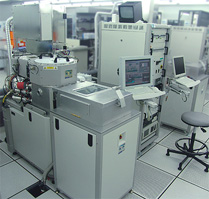
\includegraphics[width=\MachinePictureWidth]{pictures_machines/dry_DRIE.png}
\end{minipage}\begin{minipage}[H]{\MachineTextMiniPageWidth}
	\begin{tabular}{|p{3cm}|p{8cm}|}
		\hline
		Gases available
		&
		\makecell[l]{
			\tabitem $C_4 F_8$ \\
			\tabitem $S F_6$ \\
			\tabitem $O_2$ \\
			\tabitem $N_2$ \\
			\tabitem  $He$ \\
			\tabitem $Ar$
		} \\
		\hline
		RF power source
		&
		\makecell[l]{
			\tabitem 1x 1000W(max) at 13.56MHz for Coil electrode \\
			\tabitem 1x 300W(max) at 13.56MHz for Platen electrode
		} \\
		\hline
		Electrode coolant system
		&
		5 to 30 \degreesC \\
		\hline
		High speed turbo molecular pump
		&
		\makecell[l]{
			\tabitem Pumping speed of 1000 L/s at 36000 rpm \\
			\tabitem Fully automatic loadlock transfer system
		} \\
		\hline
		Substrate size
		&
		4" wafer \\
		\hline
	\end{tabular}

	\underline{Silicon etch}

	\begin{tabular}{|p{5cm}|p{6cm}|}
		\hline
		Minimum Line/Space
		&
		0.5 \um
		\\
		\hline
		Low Rate Silicon Etch E/R
		&
		From 50nm/cycle \\
		\hline
		Normal Rate Silicon Etch E/R
		&
		Up to 2 \um/min\\
		\hline
		Selectivity to Photoresist
		&
		>50:1 \\
		\hline
		Selectivity to Oxide
		&
		>80:1 \\
		\hline
		Uniformity
		&
		7\percent \\
		\hline
	\end{tabular}
\end{minipage}
